\chapter{Πυρηνική Αστροφυσική}
\label{apx:nucleosynthesis}

\section{Πυρηνοσύνθεση βαρέων στοιχείων}
Στην πυρηνική αστροφυσική, ο όρος "βαρέα στοιχεία" αναφέρεται στους πυρήνες που εντοπίζονται μετά την ομάδα του σιδήρου καθώς γι' αυτούς τους πυρήνες τα πράγματα αλλάζουν δραματικά. Γνωρίζουμε από παρατηρήσεις ότι ο σίδηρος\footnote{Στην πραγματικότητα, το $^{62}$Ni είναι αυτό με τη μεγαλύτερη ενέργεια σύνδεσης (M. P. Fewell. "\textit{The atomic nuclide with the highest mean binding energy}". American Journal of Physics, 63:653–658, July 1995). Ο Fe$^{56}$ όμως έχει μικρότερη μάζα ανα νουκλεόνιο, σε σχέση με το νικέλιο, λόγω του ότι έχει λιγότερα νετρόνια και αυτό του δίνει το "προβάδισμα" έναντι του Ni$^{62}$ όσον αφορά την ευστάθεια του πυρήνα.} έχει την μεγαλύτερη ενέργεια σύνδεσης ανα νουκλεόνιο και από εκεί και πέρα μειώνεται συνεχώς (σχήμα \ref{fig:apx:binding_energy_per_nucleon}) καθιστώντας έτσι την διαδικασία της φωτοδιάσπασης --χρησιμοποιώντας ενεργειακά κριτήρια-- μη-ευνοϊκή. Επιπρόσθετα, το συνεχώς αυξανόμενο φράγμα Coulomb μειώνει την πιθανότητα εμφάνισης του φαινομένου σήραγγος και άρα η πυρηνοσύνθεση που οφείλεται σε επαγωγή φορτισμένων σωματιδίων σταματά με την καύση του πυριτίου. Σε αντίθετη περίπτωση, οι αναμενόμενες πυρηνικές αναλογίες θα ήταν πολύ μικρότερες από αυτές που παρατηρούμε (Χ. Ελευθεριάδης, \textit{Πυρηνοσύνθεση: Δημιουργία των Στοιχείων στο Σύμπαν}, pp. 46). Με λίγα λόγια, όσον αφορά την αστρική πυρηνοσύνθέση, πυρήνες με μαζικό αριθμό μεγαλύτερο του 56 δεν μπορούν να σχηματιστούν μέσω θερμοπυρηνικών αντιδράσεων (π.χ. πυρηνική σύντηξη) και άλλοι μηχανισμοί πρέπει να ληφθούν υπόψιν.

\begin{figure}
  \centering
    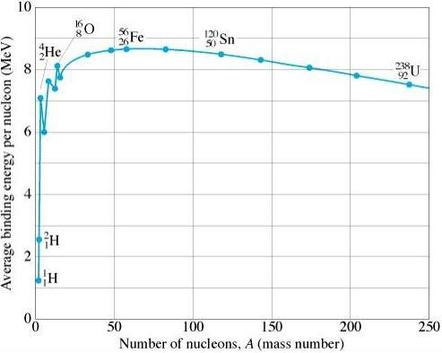
\includegraphics[scale=0.7]{Figures/benergy.jpg}
    \caption{Ενέργεια σύνδεσης ανα νουκλεόνιο συναρτήσει του μαζικού αριθμού Α.}
    \label{fig:apx:binding_energy_per_nucleon}
\end{figure}

Για την πυρηνοσύνθεση των βαρέων στοιχείων (βαρύτερων του σιδήρου) και την ερμηνεία των παρατηρούμενων ισοτοπικών αναλογιών οι Burbidge, Burbidge, Fowler και Hoyle πρότειναν το 1957 (το περίφημο B$^2$FH paper) ότι τα στοιχεία αυτά πρέπει να παράγονται κυρίως με αντιδράσεις αρπαγής νετρονίων και συνεπακόλουθες β-διασπάσεις (E. Margaret Burbidge, G. R. Burbidge, William A. Fowler, and F. Hoyle. \textit{Synthesis of the elements in stars}. Rev. Mod. Phys., 29:547–650, Oct 1957).
%% --------------------------------------------------------------------------------------------------------%%
%% --------------------------------------------------------------------------------------------------------%%
%% --------------------------------------------------------------------------------------------------------%%
\subsection{Αρπαγή νετρονίων}
Με τον όρο "αρπαγή νετρονίων" εννοούμε την πυρηνική αντίδραση κατά την οποία ένα ή περισσότερα νετρόνια συγκρούονται και "απορροφούνται" από τον πυρήνα προς σχηματισμό ενός βαρύτερου πυρήνα. Η αρπαγή νετρονίων αποτελεί την πιο απλή περίπτωση περιγραφής πυρηνικών αντιδράσεων λόγω της απουσίας δυνάμεων Coulomb. Η αντίδραση αυτή παίζει σημαντικότατο ρόλο, όπως θα δούμε παρακάτω, στην πυρηνοσύνθεση βαρέων στοιχείων στα άστρα μέσω δύο βασικών διεργασιών, την αργή διαδικασία (slow-process) και την γρήγορη διαδικασία (rapid-process). Οι όροι προέρχονται από την συσχέτιση του μέσου χρόνου που απαιτείται σε δεδομένο αστρικό περιβάλλον για αρπαγή νετρονίου, με το μέσο χρόνο ζωής του υπάρχοντος πυρήνος με β-διάσπαση (Χ. Ελευθεριάδης, \textit{Πυρηνοσύνθεση: Δημιουργία των Στοιχείων στο Σύμπαν}, pp. 47). 

Υποθέτοντας ότι η ενεργός διατομή για αρπαγή νετρονίου είναι ανεξάρτητη της ενέργειας, τότε ο μέσος χρόνος που απαιτείται για να γίνει η αρπαγή είναι:

\begin{eqnarray}
\label{eq:apx:mean_time_neutron_capture}
\tau_n = \frac{1}{N_n \langle \sigma u \rangle}\approx \frac{1}{N_n \langle \sigma \rangle u_T} = \frac{1}{N_n \langle \sigma \rangle} \left ( \frac{\mu_n}{2kT} \right )^{1/2} 
\end{eqnarray}     
όπου  $N_n$ το πλήθος των νετρονίων, $\langle \sigma \rangle$ η μέση ενεργός διατομή για σύλληψη νετρονίων, $u_T$ η ταχύτητα των θερμικών νετρονίων και $\mu_n$ η ανηγμένη μάζα των νετρονίων. Για μια τυπική ενεργό διατομή νετρονίων της τάξης των $\langle \sigma \rangle \ \sim 10^{-25}$ cm$^2$ και θερμοκρασίας των $5 \times 10^8 \,\text{K}$, προκύπτει ότι $\tau_n \approx 10^9/N_n$ χρόνια.

Ακόμα, ο μέσος χρόνος για μία β-διάσπαση όπως φαίνεται στην εξίσωση \eqref{eq:apx:beta_decay_reaction}, είναι της τάξης των μερικών ωρών.

\begin{eqnarray}
\label{eq:apx:beta_decay_reaction}
(Z, A+1) \longrightarrow (Z+1, A+1) + e^{-} + \overline{\nu}_e
\end{eqnarray}
%% --------------------------------------------------------------------------------------------------------%%
%% --------------------------------------------------------------------------------------------------------%%
%% --------------------------------------------------------------------------------------------------------%%
\subsubsection{Η s-διεργασία}
Ας υποθέσουμε ένα αστρικό περιβάλλον στο οποίο η πυκνότητα των νετρονίων είναι χαμηλή, $N_n \sim 10^5 $ cm$^{-3}$, και άρα ο χρόνος που απαιτείται για να γίνει σύλληψη νετρονίου από έναν πυρήνα είναι μεγάλος. Μέσα σε αυτό το χρονικό διάστημα, ο πυρήνας θα κάνει αρπαγή ενός νετρονίου και ταυτόχρονα θα εκπέμψει ένα φωτόνιο σύμφωνα με την αντίδραση

\begin{eqnarray}
\label{eq:apx:neutron_capture_reaction}
(Z, A) + n \longrightarrow (Z, A+1) + \gamma
\end{eqnarray}
Το ισότοπο που θα προκύψει μπορεί να είναι είτε σταθερό, είτε ασταθές. Εάν είναι σταθερό τότε, μέσω της ίδιας διαδικασίας, θα δημιουργηθεί ένα νέο ισότοπο $(Z, A+2)$ κοκ. Στην περίπτωση όμως που το ισότοπο που δημιουργείται είναι ασταθές όσον αφορά τη β-διάσπαση (λόγω περισσείας νετρονίων), τότε θα διασπαστεί πριν προλάβει να λάβει χώρα η επόμενη αρπαγή νετρονίου και το ισότοπο που θα δημιουργηθεί θα είναι το $(Z+1, A+1)$ οδεύοντας με αυτό τον τρόπο προς την κοιλάδα σταθερότητας. Αυτή είναι η λεγόμενη \textbf{s-διεργασία} και συμβαίνει όταν ο χρόνος διάσπασης ενός ασταθούς πυρήνα είναι μικρότερος από τον χρόνο που απαιτείται για να κάνει αρπαγή νετρονίου. Τα ισότοπα που εξελίσσονται βάσει αυτής της διεργασίας βρίσκονται επάνω ή πολύ κοντά στην κοιλάδα σταθερότητας, οπότε η s-διεργασία είναι υπεύθυνη για την παραγωγή της πλειονότητας των στοιχείων με μαζικό αριθμό από 63 εως 209 καθώς ο $^{209}$Bi είναι ο πιο βαρύς σταθερός πυρήνας. Το ισότοπο με $A=210$ παράγεται με νετρονική αρπαγή από το $^{209}$Bi και διασπάται με α-εκπομπή στο $^{206}$Pb, έτσι ένας μικρός κύκλος που αποτελείται από μια αρπαγή νετρονίου και μια εκπομπή σωματιδίου άλφα τερματίζει την s-διεργασία\footnote{Πλήρης ανάλυση για τον τερματισμό της s-διεργασίας μπορεί να βρεθεί στο paper των Clayton και Rassbach, \textit{Termination of the s-Process}, \textit{The Astrophysical Journal, Vol. 148, April 1967.}} (D. Clayton, \textit{Principles of Stellar Evolution and Nucleosynthesis}, McGraw-Hill Book Company, New York, 1968, pp. 560).

\begin{figure}
    \centering
    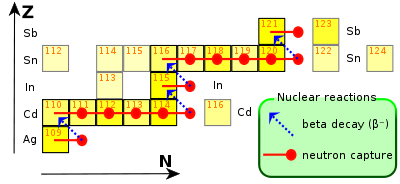
\includegraphics[scale=0.7]{Figures/sprocess.png}
    \caption{Η διαδρομή της s-διεργασίας.}
    \label{fig:apx:sprocess_path}
\end{figure}
%% --------------------------------------------------------------------------------------------------------%%
%% --------------------------------------------------------------------------------------------------------%%
%% --------------------------------------------------------------------------------------------------------%%
\subsubsection{Η r-διεργασία}
Στη συνέχεια ας αναλογιστούμε ένα διαφορετικό περιβάλλον όπου η ροή των νετρονίων είναι πολύ υψηλή, $N_n \sim$ $10^{23} \,\text{cm}^{-3}$. Τόσο υψηλές ροές νετρονίων παρατηρούνται κατά την έκρηξη υπερκαινοφανών αστέρων (supernovae). Σε αυτό το σενάριο, έχουμε διαδοχικές συλλήψεις νετρονίων σε πολύ μικρή χρονική κλίμακα, της τάξης των millisecond, και έτσι τα ενδιάμεσα ισότοπα δεν προλαβαίνουν να διασπασθούν οπότε δημιουργούνται πυρήνες εξαιρετικά πλούσιοι σε νετρόνια. Οι πυρήνες αυτοί εντοπίζονται μακριά από την κοιλάδα σταθερότητας και συνεπώς αυξάνεται η αστάθεια τους όσο αυξάνεται ο αριθμός των νετρονίων που συλλαμβάνουν. Φυσικά υπάρχει ένα ανώτατο όριο στο πόσο μπορεί να αυξηθεί ο αριθμός των νετρονίων στα διάφορα στοιχεία. Το όριο αυτό ονομάζεται \textbf{neutron drip line} και είναι το όριο στο οποίο η ενέργεια σύνδεσης του τελευταίου νετρονίου μηδενίζεται. 
Όσο πλησιάζουμε αυτό το όριο, οι πυρήνες γίνονται όλο και πιο ασταθείς και ο μέσος χρόνος που απαιτείται για να πραγματοποιηθεί μία β-διάσπαση γίνεται συγκρίσιμος με τον μέσο χρόνο που απαιτείται για να γίνει μία αρπαγή νετρονίου. Έτσι, καθίσταται δυνατόν να προηγηθεί μία β-διάσπαση από μία σύλληψη νετρονίου οπότε ο πυρήνας κάνει ένα βήμα προς την κοιλάδα σταθερότητας. Το στοιχείο όμως που δημιουργήθηκε από την β-διάσπαση δεν προχωράει περαιτέρω καθώς είναι πιο σταθερό από το μητρικό του και άρα ο μέσος χρόνος διάσπασης του είναι μεγαλύτερος από τον αντίστοιχο της αρπαγής νετρονίων. Πρέπει να περιμένουμε λοιπόν μέχρι να δημιουργηθεί ξανά ένα εξόχως βραχύβιο ισότοπο το οποίο με την σειρά του θα κάνει το δικό του βήμα προς τη κοιλάδα σταθερότητας κοκ. 
Στην περίπτωση που δημιουργηθεί ένα ισότοπο με μαγικό αριθμό νετρονίων (κλειστοί νετρονικοί φλοιοί), εμφανίζει μεγάλη αντίσταση στην αρπαγή νετρονίων καθώς τείνει να διασπαστεί αμέσως. Όταν όμως υπάρχει μεγάλη ροή νετρονίων δεν είναι απίθανο να γίνουν διαδοχικές συλλήψεις πριν προλάβει να διασπαστεί και έτσι να συνεχιστεί η r-διεργασία. Οι κορυφές όπου δημιουργούνται στοιχεία με κλειστούς νετρονικούς φλοιούς καθώς και η επίδραση που έχουν στην εξέλιξη της r-διεργασίας φάινεται στο σχήμα \ref{fig:apx:rprocess_path}.
Η διαδικασία αυτή ονομάζεται \textbf{r-διεργασία} και συμβαίνει όταν ο μέσος χρόνος διάσπασης ενός πυρήνα είναι μεγαλύτερος από τον μέσο χρόνο στον οποίο κάνει αρπαγή νετρονίων. Ο τερματισμός της διεργασίας αυτής πραγματοποιείται μέσω φαινομένων σχάσης.

\begin{figure}
    \centering
    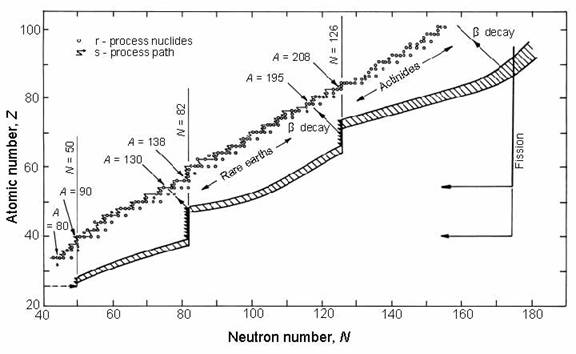
\includegraphics[scale=0.7]{Figures/processes.jpg}
    \caption{Η διαδρομή της r-διεργασίας. Η διαφορά της με την s-διεργασία είναι εμφανής καθώς φαίνεται ο τρόπος που απομακρύνεται από την κοιλάδα σταθερότητας. Τα κάθετα "σκαλοπατάκια" που εμφανίζονται στο διάγραμμα αντιστοιχούν σε μαγικούς αριθμούς όπου η r-διεργασία εμφανίζει ισχυρή αντίσταση.}
    \label{fig:apx:rprocess_path}
\end{figure}

Είναι φανερό ότι, μόλις σταματήσει η ακτινοβόληση με νετρόνια, τα r-ισότοπα που έχουν δημιουργηθεί θα αρχίσουν να υπόκεινται σε β-διασπάσεις --όντας ασταθή-- λόγω του δυσανάλογα μεγάλου αριθμού νετρονίων που έχουν. Γενικά, μπορούμε να έχουμε την παραγωγή ισοτόπων και με τις δύο διεργασίες που έχουμε αναφέρει μέχρι στιγμής, όπως επίσης και ισότοπα που προέρχονται αποκλειστικά μόνο από μία από αυτές. Αν για παράδειγμα, ένας r-πυρήνας καταλήξει μετά από τις διαδοχικές β-διασπάσεις σε σταθερό ισότοπο $(Z, A)$, τότε αν το επόμενο ισότοπο $(Z+1, A)$ είναι επίσης σταθερό, πρέπει αναγκαστικά να έχει δημιουργηθεί με την s-διεργασία και όχι με την r. 
Το τελικό αποτέλεσμα στις αναλογίες των στοιχείων είναι να έχουμε ισότοπα που προέρχονται στην πλειοψηφία τους από την s-διεργασία αλλά και ισότοπα που προέρχονται αποκλειστικά από την r-διεργασία. Οι κοσμικές αναλογίες των βαρέων στοιχείων φαίνονται στο σχήμα \ref{fig:apx:cosmic_abundances}.


Έχοντας εξασφαλίσει μία βασική γνώση για τον τρόπο δημιουργίας των βαρέων στοιχείων σε διάφορες αστρικές συνθήκες, μπορούμε να κάνουμε κάποιες βασικές παρατηρήσεις. Όπως αναφέρει ο Clayton στο βιβλίο του \textit{Principles of Stellar Evolution and Nucleosynthesis}, η σύνθεση βαρέων στοιχείων μέσω της s-διεργασίας μπορεί να ξεκινήσει από οποιονδήποτε πυρήνα με $A > 8$. Όμως η ενεργός διατομή για αρπαγή νετρονίου στους ελαφρείς πυρήνες είναι κατά μέσο όρο πολύ μικρότερη από την αντίστοιχη ενεργό διατομή για πυρήνες μετά την ομάδα του σιδήρου. Έτσι, απαιτείται πολύ μεγαλύτερη ροή νετρονίων για την δημιουργία ενός βαρέως πυρήνα ξεκινώντας από το πυρίτιο, για παράδειγμα, απ' ότι ξεκινώντας από το σίδηρο. Γίνεται αντιληπτό λοιπόν ότι λόγω του περιορισμένου αριθμού ελεύθερων νετρονίων που είναι διαθέσιμα, είναι πολύ πιο ωφέλιμο να έχουμε σύνθεση βαρέων στοιχείων χρησιμοποιώντας την ομάδα του σιδήρου σαν "δότες" (seed nuclei) αντί τα ελαφρύτερα στοιχεία. 

Στο σημείο αυτό, γίνεται ξεκάθαρο ότι οι αντιδράσεις και οι μηχανισμοί παραγωγής ελεύθερων νετρονίων σε ένα δεδομένο αστρικό περιβάλλον είναι μείζωνος σημασίας για την εξέλιξη της s-διεργασίας. Γενικά, τα ελεύθερα νετρόνια δεν βρίσκονται σε αφθονία κατά την διάρκεια των φάσεων καύσης των πυρηνικών καυσίμων ενός αστέρα όπως περιγράφηκαν στο κεφάλαιο 3. Γι' αυτό το λόγο είναι σημαντική η ύπαρξη αναλυτικών μοντέλων αστρικής εξέλιξης ώστε να γίνει κατανοητή η πηγή αυτών των νετρονίων. Σήμερα, θεωρείται παραδεκτό ότι η κύρια πηγή ελεύθερων νετρονίων προέρχεται από αρπαγές σωματιδίων-α στα διάφορα στρώματα φλοιών ενός αστέρα σύμφωνα με τις αντιδράσεις:

\begin{eqnarray}
\rm C^{13}  &(\alpha, n)&  \rm O^{16} \label{eq:apx:c13+alpha_o16+n}\\
\rm O^{17}  &(\alpha, n)&  \rm Ne^{20} \label{eq:apx:o17+alpha_ne20+n}\\
\rm Ne^{21}  &(\alpha, n)& \rm Mg^{24} \label{eq:apx:ne21+alpha_mg24+n}
\end{eqnarray}
όπου η \eqref{eq:apx:o17+alpha_ne20+n} είναι η πιο πολλά υποσχόμενη από αυτές, απλά γιατί το O$^{17}$ φαίνεται να παράγεται και να υπάρχει σε μεγαλύτερη αφθονία σε σχέση με τα άλλα δύο.    

Το τελικό συμπέρασμα που πρέπει να κρατήσουμε για την s-διεργασία είναι ότι: 

\begin{itemize}
\item γίνεται στο εσωτερικό των άστρων.
\item απαιτεί μικρή ροή ελεύθερων νετρονίων ώστε τα ασταθή ισότοπα που προκύπτουν να προλαβαίνουν να υποστούν β-διάσπαση.
\item μπορούμε να υποθέσουμε ρεαλιστικά ότι τροφοδοτείται από την ομάδα του σιδήρου.
\item λαμβάνει χώρα κοντά στη κοιλάδα σταθερότητας και δημιουργεί ισότοπα με κλειστούς νετρονικούς φλοιούς.
\end{itemize}


Αντίστοιχα τα βασικά σημεία που πρέπει να μας μείνουν σχετικά με την r-διεργασία είναι:

\begin{itemize}
\item γίνεται κατά τα τελευταία στάδια πριν την καταστρεπτική έκρηξη ενός υπερκαινοφανούς αστέρα (supernova).
\item απαιτεί πολύ μεγάλη ροή ελεύθερων νετρονίων ώστε τα ασταθή ισότοπα που προκύπτουν να μην προλαβαίνουν να υποστούν β-διάσπαση. Τέτοιες συνθήκες κυριαρχούν στα supernovae.
\item λαμβάνει χώρα μακριά από τη κοιλάδα σταθερότητας και είναι υπεύθυνη για ισότοπα ιδαιτέρως πλούσια σε νετρόνια.
\item  Τα τελικά σταθερά ισότοπα που δημιουργούνται έχουν νετρονικό αριθμό μικρότερο του αντιστοιχούντος σε κλειστό νετρονικό φλοιό.
\end{itemize}


\begin{figure}
    \centering
    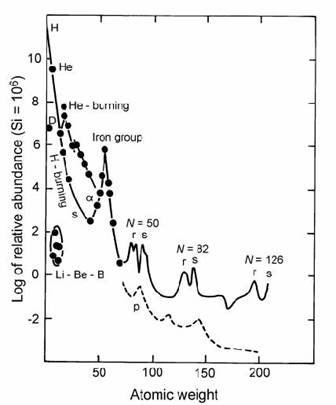
\includegraphics[scale=0.7]{Figures/abundance.jpg}
    \caption{Κοσμικές αναλογίες των βαρέων στοιχείων συναρτήσει του μαζικού αριθμού. Σημαντική λεπτομέρεια ότι οι κορυφές αριστερά των αντιστοιχουσών σε κλειστούς νετρονικούς φλοιούς (Ν=50, 82, 126) οφείλονται σε ισότοπα προερχόμενα από την r-διεργασία.}
    \label{fig:apx:cosmic_abundances}
\end{figure}
%% --------------------------------------------------------------------------------------------------------%%
%% --------------------------------------------------------------------------------------------------------%%
%% --------------------------------------------------------------------------------------------------------%%
\subsection{Αρπαγή πρωτονίων}
Μέχρι στιγμής είδαμε το πως μπορούν να δημιουργηθούν πυρήνες πλούσιοι σε νετρόνια, μέσω της αρπαγής νετρονίων. Υπάρχουν όμως και κάποιοι πυρήνες, πλούσιοι σε πρωτόνια, η παρουσία των οποίων δεν μπορεί να ερμηνευθεί με καμία διαδικασία σύλληψης νετρονίων. Ένας τρόπος δημιουργίας τέτοιων πυρήνων είναι η αρπαγή πρωτονίου προς σχηματισμό βαρύτερων ισοτόπων για την οποία θα μιλήσουμε σε αυτό το υποκεφάλαιο. Οι πυρήνες οι οποίοι είναι πλούσιοι σε πρωτόνια και δεν μπορούν να παραχθούν μέσω της s ή της r-διεργασίας, ονομάζονται \textbf{p-πυρήνες}.
%% --------------------------------------------------------------------------------------------------------%%
%% --------------------------------------------------------------------------------------------------------%%
%% --------------------------------------------------------------------------------------------------------%%
\subsubsection{Η p-διεργασία}
Ο όρος p-διεργασία παρουσιάζεται για πρώτη φορά στο διάσημο B$^2$FH paper στο οποίο προτείνεται σαν ο μοναδικός μηχανισμός παραγωγής p-πυρήνων σε υπερκαινοφανείς αστέρες τύπου ΙΙ (type-II supernovae). Αργότερα, αποδείχτηκε ότι δεν πληρούνται οι συνθήκες σε τέτοιου είδους υπερκαινοφανών.
Η διεργασία έχει ως αφετηρία τα βαρέα ισότοπα τα οποία προήλθαν από την s ή την r διεργασία. Στη συνέχεια, ένα πρωτόνιο συλλαμβάνεται μέσω της γενικής αντίδρασης $(p, \gamma)$, αλλάζοντας έτσι το ισότοπο σ' ένα καινουργιο χημικό στοιχείο ενώ ταυτόχρονα, αλλάζει και ο λόγος νετρονίων-πρωτονίων οδηγώντας μας έτσι σε πυρήνες πλούσιους σε πρωτόνια.

Είναι φανερό ότι η λογική αυτή δεν θα οδηγήσει σε πολύ βαρείς πυρήνες λόγω του ότι η θερμοκρασία του πλάσματος δεν αυξάνει αυθαίρετα με αποτέλεσμα τα πρωτόνια να μην έχουν την κατάλληλη ενέργεια για να ξεπεράσουν το συνεχώς αυξανόμενο φράγμα Coulomb. Αλλά ακόμα κι αν η θερμοκρασία αυξάνονταν με αυθαίρετο τρόπο, οι επικείμενες φωτοδιασπάσεις δεν θα επέτρεπαν τον σχηματισμό βαρέων πυρήνων επειδή θα αφαιρούσαν πρωτόνια με πιο γρήγορο ρυθμό από τις αρπαγές πρωτονίων. Ένας εναλλακτικός τρόπος από την p-διεργασία θα μπορούσε να γίνει σ' ένα περιβάλλον όπου υπάρχει υπερβολικά μεγάλη ροή πρωτονίων με αποτέλεσμα να αυξάνεται ο ρυθμός των αρπαγών χωρίς να χρειαστεί να αυξηθεί σημαντικά η θερμοκρασία του πλάσματος. Τέτοιους μηχανισμούς θα εξετάσουμε στη συνέχεια.
%% --------------------------------------------------------------------------------------------------------%%
%% --------------------------------------------------------------------------------------------------------%%
%% --------------------------------------------------------------------------------------------------------%%
\subsubsection{Η rp-διεργασία}
Η συγκεκριμένη διαδικασία παίρνει το όνομά της από τον όρο "\textbf{ταχεία σύλληψη πρωτονίου}" (rapid proton capture process) και είναι προφανές ότι απαιτεί συγκεκριμένες συνθήκες ροής πρωτονίων και θερμοκρασίας προκειμένου να ξεπεραστεί το φράγμα Coulomb. Τέτοιες συνθήκες πιστεύεται ότι υπάρχουν σε διπλά συστήματα αστέρων, που αποτελούνται συνήθως από έναν αστέρα νετρονίων και έναν συνοδό αστέρα\footnote{Τα συστήματα αυτά ονομάζονται αλλιώς και x-ray bursters.}. Σ' ένα τέτοιο σύστημα, αστρική ύλη από το συνοδό αστέρα έλκεται από το έντονο βαρυτικό πεδίο του αστέρα νετρονίων και δημιουργείται έτσι ένας περιστρεφόμενος δίσκος συσσώρευσης (accretion disk). Με αυτό τον τρόπο ενεργοποιείται μία εκρηκτική καύση υδρογόνου στα πλαίσια της οποίας εξελίσσεται και η rp-διεργασία. Δεν είναι απίθανο να έχουμε παρόμοια φαινόμενα και στον δίσκο συσσώρευσης γύρω από μία μαύρη τρύπα (R. Surman ,et.al., \textit{Heavy element synthesis in neutrino-processed black hole accretion disk ejecta}, Proceedings of Science, XIII Nuclei in the Cosmos, 7-11 July 2014, Debrecen, Hungary).
Λόγω της συνεχούς αύξησης των πρωτονίων, η διαδικασία αυτή οδηγεί σε παραγωγή ισοτόπων που απομακρύνονται από την κοιλάδα σταθερότητας και πλησιάζουν προς την λεγόμενη \textbf{proton drip line} η οποία ορίζεται σε αντιστοιχία με την neutron drip line. Όσο πλησιάζουμε σε αυτό το όριο, οι άλφα διασπάσεις, η β$^{+}$ διάσπαση καθώς και η εκπομπή πρωτονίου γίνονται όλο και πιο συχνές και οδηγούν τα ασταθή ισότοπα πίσω προς την κοιλάδα σταθερότητας. Το τελευταίο ισότοπο το οποίο μπορεί να παράγει αυτή η διεργασία είναι το Te $^{107}$ το οποίο τείνει να διασπαστεί με α-διάσπαση, οπότε κλείνει με αυτόν τον τρόπο ο κύκλος της rp-διεργασίας.
%% --------------------------------------------------------------------------------------------------------%%
%% --------------------------------------------------------------------------------------------------------%%
%% --------------------------------------------------------------------------------------------------------%%
\subsubsection{Η pn-διεργασία}
Μία ακόμα διεργασία η οποία μπορεί να συμβαίνει παράλληλα με την rp-process είναι η λεγόμενη \textbf{pn-διεργασία} (neutron-rich rapid proton capture) και πρόκειται ουσιαστικά για αντιδράσεις τύπου $(n, p)$. Μέσω των αντιδράσων αυτών μπορεί εύκολα να ξεπεραστούν τα σημεία αναμονής (waiting points)\footnote{Όταν ένας πυρήνας δεν μπορεί να προχωρήσει παρακάτω προς σχηματισμό βαρύτερου ισοτόπου είτε λόγω φωτοδιασπάσεων, είτε λόγω προσέγγισης στη drip line, τότε πρέπει να περιμένει μέχρι να β-διασπαστεί ή μέχρι να βρεθεί τρόπος να "ξεφύγει" από αυτό το σημείο μέσω κάποιας διαδικασίας. Τα σημεία αυτά στα οποία κάποια ισότοπα φαίνεται να "περιμένουν" για την εξέλιξη της πυρηνοσύνθεσης ονομάζονται σημεία αναμονής.} της rp-διεργασίας καθώς ο χρόνος για μια τέτοια αντίδραση είναι μικρότερος τόσο από τον μέσο χρόνο αρπαγής πρωτονίου/φωτοδιάσπασης όσο και από τον μέσο χρόνο β-διάσπασης στα σημεία αυτά.
Φυσικά, αυτός ο μηχανισμός απαιτεί μία πηγή ελεύθερων νετρονίων τα οποία δεν είναι συνήθως παρόντα σε περιβάλλον με τόσο πυκνό πλάσμα πρωτονίων.
%% --------------------------------------------------------------------------------------------------------%%
%% --------------------------------------------------------------------------------------------------------%%
%% --------------------------------------------------------------------------------------------------------%%
\subsubsection{Η $\nu$p-διεργασία}
Το 2006 προτάθηκε από την Fr\"ohlich και άλλους (C. Fr\"ohlich, et.al., \textit{Neutrino-induced nucleosynthesis of A $\geq$ 64 nuclei: The $\nu$p process}, Phys. Rev. Lett., 96:142502, Apr 2006) ένας καινούργιος μηχανισμός παραγωγής νετρονίων σε περιβάλλον πλούσιο σε πρωτόνια μέσω της αντίδρασης:

\begin{equation}
\overline{\nu}_e + p \longrightarrow e^{+} + n
\end{equation}

Αυτός ο μηχανισμός ομάστηκε \textit{$\nu$p-διεργασία} και θα μπορούσε να παρέχει τα απαραίτητα νετρόνια για την εξέλιξη της pn-διεργασίας σε ένα περιβάλλον όπου εκτός από την παρουσία πλάσματος με μεγάλη πυκνότητα πρωτονίων, θα υπάρχει επίσης και μεγάλη ροή (αντι)-νετρίνων καθώς τα τελευταία αλληλεπιδρούν εξαιρετικά ασθενώς με την ύλη. Τέτοιες συνθήκες πιστεύεται ότι επικρατούν σε υπερκαινοφανείς αστέρες και σε εκλάμψεις ακτίνων γαμμα (gamma-ray bursts).
%% --------------------------------------------------------------------------------------------------------%%
%% --------------------------------------------------------------------------------------------------------%%
%% --------------------------------------------------------------------------------------------------------%%
\subsection{Φωτοδιάσπαση}
Είδαμε πως μπορεί να δημιουργηθεί ένας πυρήνας πλούσιος σε πρωτόνια μέσω της συλλήψης πρωτονίου. Ένας δεύτερος τρόπος δημιουργίας τέτοιων πυρήνων είναι η \textbf{φωτοδιάσπαση} ή αλλιώς \textbf{γ-διεργασία}, κατά την οποία έχουμε μείωση του αριθμού των νετρονίων από έναν πυρήνα μέσω αντιδράσεων τύπου (γ,n). Γενικά, στις συνθήκες υψηλής ενέργειας που μελετάμε, το φαινόμενο της φωτοδιάσπασης εμφανίζεται πολύ συχνά και εμποδίζει κατά κάποιον τρόπο τους πυρήνες να φτάσουν στις drip lines. 
Φαίνεται ότι η φωτοδιάσπαση και η αρπαγή πρωτονίου είναι ανταγωνιστικοί μεταξύ τους μηχανισμοί δημιουργίας βαρέων πυρήνων και σήμερα είναι γενικά αποδεκτό ότι η φωτοδιάσπαση είναι η βασική διαδικασία σύνθεσης p-πυρήνων.
%% --------------------------------------------------------------------------------------------------------%%
%% --------------------------------------------------------------------------------------------------------%%
%% --------------------------------------------------------------------------------------------------------%%
\subsection{Η l-διεργασία}
Όπως έχει αναφερθεί, η ύπαρξη των ελαφρών στοιχείων όπως το λίθιο, το δευτέριο, το βόριο και το βηρύλλιο, δεν δικαιολογείται λόγω των συνθηκών που επικρατούν στο εσωτερικό των άστρων. Σε αυτές τις συνθήκες, τα στοιχεία αυτά θα έπρεπε να καταστρέφονται πολύ γρήγορα και άρα να μην παρατηρούνται σε αυτές τις κοσμικές αναλογίες, έστω κι αν αυτές είναι πολύ μικρές. Άρα, είτε πρέπει να δημιουργήθηκαν σε ψυχρό περιβάλλον, είτε να απομακρύνθηκαν από το αστρικό περιβάλλον αμέσως μετά την δημιουργία τους. 
Ένας μηχανισμός που μπορεί να εξηγήσει τη σύνθεση αυτών των στοιχείων στο μεσοαστρικό χώρο (άρα σε ψυχρή περιοχή) είναι η \textbf{ l-διεργασία}\footnote{Στη διεθνή βιβλιογραφία μπορεί να συναντήσει κάποιος και τον όρο x-διεργασία αντί του όρου l-διεργασία.} η οποία πρόκειται ουσιαστικά για μία αντίδραση θρυμματισμού (spallation). Κατά την διαδικασία αυτή, κοσμικές ακτίνες προσπίπτουν σε στοιχεία με σημαντική κοσμική αναλογία (C, N, O) και τα διασπούν με κυρίως παράγωγα τα Li, Be και Β.

Στο περιβάλλον στο οποίο λαμβάνουν χώρα οι διαδικασίες πυρηνοσύνθεσης, δεν μπορούμε να τοποθετήσουμε κάποιον ανιχνευτή και να πάρουμε πρωτογενή δεδομένα. Γι' αυτό το λόγο δημιουργείται η ανάγκη να μπορέσουμε με κάποιο τρόπο να τις εκφράσουμε μέσω των μαθηματικών και στη συνέχεια να μπορέσουμε με την βοήθεια αριθμητικών μεθόδων να τις προσομοιώσουμε, να τις αξιολογήσουμε και να τις συγκρίνουμε με τα παρατηρησιακά μας δεδομένα. Αν θέλουμε να προσομοιώσουμε όμως την δημιουργία όλων των στοιχείων, θα πρέπει να γνωρίζουμε αρχικά όλα εκείνα τα φυσικά χαρακτηριστικά που μπορούν να την περιγράψουν. Για παράδειγμα, θα πρέπει να γνωρίζουμε τα χαρακτηριστικά των πυρήνων που μπορεί να λαμβάνουν μέρος στην πυρηνοσύνθεση, τον χρόνο ημιζωής τους, το σπιν τους, τα ενεργειακά τους επίπεδα κ.α. Πρέπει να ξέρουμε επίσης και τα χαρακτηριστικά των αντιδράσεων μεταξύ πυρήνων, νουκλεονίων, λεπτονίων, φωτονίων ή νετρίνων. 

 \begin{figure}
     \centering
     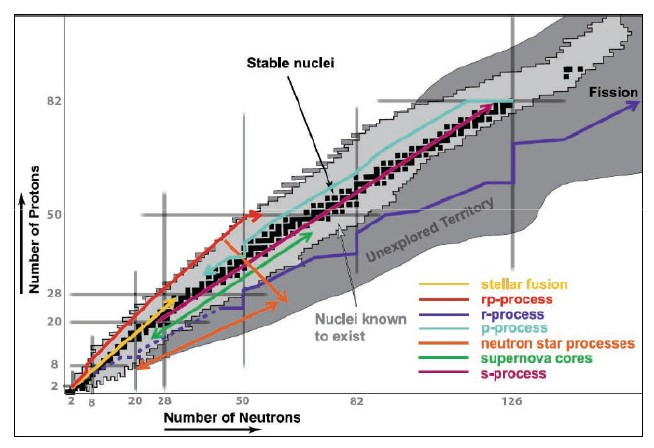
\includegraphics[scale=0.6]{Figures/Screenshot_2.jpg} 
    \caption{Διάγραμμα Segre και συσχέτιση των χημικών στοιχείων με τους μηχανισμούς παραγωγής τους.}
    \label{fig:apx:segre_diagram}
\end{figure} 

Παρακάτω θα περιγράψουμε πως μπορούμε να κατασκευάσουμε τη  διαφορική εξίσωση, που στην συνέχεια κάποιος πρέπει να επιλύσει αριθμητικά με σκοπό να προσομοιώσει τις διαδικασίες της πυρηνοσύνθεσης.  
%------------------------------------------------------------------------------------------------------------
%------------------------------------------------------------------------------------------------------------
%------------------------------------------------------------------------------------------------------------
\section{Ρυθμός Αντιδράσεων}
Aς υποθέσουμε λοιπόν ότι έχουμε στο εργαστήριό μας ένα αέριο που αποτελείται από δυο σωματίδια i και j τα οποία έχουν αριθμητικές πυκνότητες $n_{i}$ (cm$^{-3}$) και $n_{j}$ (cm$^{-3}$) με \textit{n} να είναι ο αριθμός των σωματιδίων στον όγκο και την ενεργό διατομή μεταξύ αυτων των δυο $\sigma$ (cm$^{2}$). Αρχικά και για λόγους απλότητας, θεωρούμε το ένα σωματίδιο ακίνητο, ως στόχο (έστω το σωμάτιο j), και αυτόν τον στόχο θα τον "βομβαρδίσουμε" με το άλλο σωμάτιο, το οποίο θα κινείται με γνωστή ταχύτητα. 

\begin{figure}
    \centering
    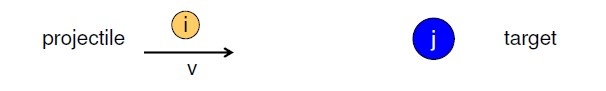
\includegraphics[scale=0.6]{Figures/target.jpg}  
    \caption{Διάταξη βλήματος-στόχου.}
    \label{fig:apx:target_projectile}
\end{figure} 

Aυτό που θα μετρήσουμε πειραματικά είναι η ενεργός διατομή μεταξύ αυτών των σωματιδίων. Οι ποσότητες που μας ενδιαφέρουν ωστόσο από αυτή την διαδικασία είναι το πόσες αντιδράσεις γίνονται στη μονάδα του χρόνου και στη μονάδα του όγκου. Η πληροφορία αυτή όμως, σχετίχεται με την σχετική ροή των σωματιδίων i, τον αριθμό των σωματιδίων j και την μετρούμενη ενεργό διατομή μεταξύ τους. Συνδυάζοντας τα παραπάνω μπορούμε να γράψουμε τις αντιδράσεις που θα πραγματοποιηθούν από αυτή την σύγκρουση των δυο σωματιδίων με τη μορφή:

\begin{equation}
\label{eq51}
r = n_{i}\cdot u \cdot n_{j}\cdot \sigma (u) \ \text{cm}^{-3}\text{/s}
\end{equation}
Στη Φύση όμως είναι σχεδόν απίθανο να βρεθεί ένα σωματίδιο ακίνητο. Το πιθανότερο σενάριο είναι και τα δυο σωμάτια να βρίσκονται σε κίνηση τη στιγμή της μεταξύ τους σύγκρουσης. Έτσι, για να εκφράσουμε  και αυτή την κίνηση του δεύτερου σωματίου θα πρέπει να υπολογίσουμε την σχετική ταχύτητα μεταξύ τους. Πλέον λοιπόν, οι αντιδράσεις ανά μονάδα χρόνου και όγκου θα είναι:

\begin{equation}
\label{eq52}
r_{i,j}= \int \sigma\cdot \vert \vec{u_{i}}- \vec{u_{j}} \vert dn_{i}dn_{j}
\end{equation}
Γενικά όμως, τα σωματίδια δεν έχουν σταθερή ταχύτητα κατά τη διάρκεια της κίνησής τους αλλά παρουσιάζουν μια κατανομή ταχυτήτων, έτσι είναι αναγκαίο να συμπεριλάβουμε και αυτή την παράμετρο γράφοντας:

\begin{equation}
\label{eq53}
r_{i,j}= \int \sigma( \vert \vec{u_{i}}- \vec{u_{j}} \vert) \cdot \vert \vec{u_{i}}- \vec{u_{j}} \vert \cdot \phi(\vec{u_{i}}) \cdot \phi(\vec{u_{j}})d^{3}u_{i}d^{3}u_{j}
\end{equation}
όπου το $r_{i,j}$ εκφράζει τον ρυθμό των αντιδράσεων, το $\sigma( \vert \vec{u_{i}}- \vec{u_{j}} \vert)$ την ενεργό διατομή συναρτήσει της σχετικής ταχύτητας μεταξύ των δυο σωματιδίων, το $\vert \vec{u_{i}}- \vec{u_{j}} \vert $ την σχετική ταχύτητα μεταξύ των δυο σωματιδίων και τέλος τα $\phi(\vec{u_{i}}), \phi(\vec{u_{j}})$ την κατανομή των ταχυτήτων με τις οποίες κινούνται τα σωματίδια.
Το πρόβλημά μας όμως ακόμα δεν έχει παραμετροποιηθεί πλήρως. Οι πυρήνες που βρίσκονται μέσα στο αστροφυσικό πλάσμα ενός αστέρα για παράδειγμα, δεν έχουν όλοι την ίδια ενέργεια. Ακολουθούν μια κατανομή ενεργειών και πιο συγκεκριμένα μπορούμε να εκφράσουμε αυτή την πληθώρα ενεργειών μεσω της γνωστής μας κατανομής Maxwell-Boltzmann.

\begin{figure}[h]
    \centering
    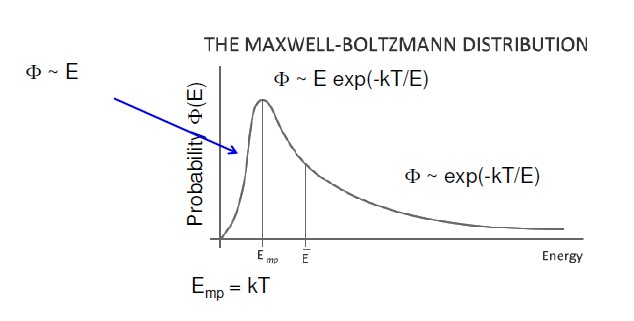
\includegraphics[scale=0.7]{Figures/mb.jpg} 
    \caption{Κατανομή Maxwell-Boltzmann.}
    \label{fig:apx:mb}
\end{figure} 
Η κατανομή Maxwell-Boltzmann όπως βλέπουμε και στο σχήμα \ref{fig:apx:mb}, στον οριζόντιο άξονα εκφράζει την ενέργεια και στον κάθετο άξονα εκφράζει την πιθανότητα να συναντήσουμε αυτή την ενέργεια στο σύστημα που μελετάμε. Παρατηρούμε ότι το μέγιστο της κατανομής εμφανίζεται σε περιοχή χαμηλών ενεργειών ενώ μια μακριά και φθίνουσα ουρά αντιστοιχεί σε μεγαλύτερες τιμές ενέργειας. Για να μπορέσουμε να κάνουμε ένα βήμα παραπέρα πάνω στην προσομοίωση της πυρηνοσύνθεσης, θα πρέπει να κάνουμε κάποιες απαραίτητες απλοποιήσεις. Ορίζουμε λοιπόν ως κέντρο αυτού του συστήματος το κέντρο μάζας του σωματιδίου που μελετάμε λαμβάνοντας υπόψιν ότι η κατανομή των ταχυτήτων κανονικοποιείται στη μονάδα

\begin{equation}
\label{eq54}
\int \phi \left( \vec{u}  \right) d^{3}u = 1
\end{equation} 
και κανονικοποιούμε την κατανομή πιθανότητας ενεργειών συναρτήσει του όγκου. Έπειτα από τα παραπάνω ο ρυθμός αντίδρασης έχει πλέον την μορφή

\begin{equation}
\label{eq55}
r_{i,j}=n_{i}n_{j}\langle \sigma u \rangle_{i,j}
\end{equation}
όπου ο όρος $\langle \sigma u \rangle_{i,j}$ εκφράζει την μέση θερμοπυρηνική ενεργό διατομή. Αν θέλουμε τώρα να υπολογίσουμε την θερμοπυρηνική ενεργό διατομή για σωματίδια που ανήκουν σε όλο το ενεργειακό φάσμα που φαίνεται στην κατανομή Maxwell-Boltzmann, λαμβάνοντας υπόψιν τα προηγούμενα βήματα, καταλήγουμε στη σχέση:
\begin{equation}
\label{eq56}
\langle \sigma u \rangle (T) = \left(  \frac{8}{\mu \pi} \right)^{1/2} \frac{1}{kT^{3/2}} \int_{0}^{\infty} E \sigma(E) \exp (-E/kT)dE
\end{equation}
όπου $\mu$ το χημικό δυναμικό του συστήματος που μελετάμε, Τ η θερμοκρασία, $\sigma(E)$ η ενεργός διατομή των ταχυτήτων συναρτήσει της ενέργειας και k η σταθερά Maxwell-Boltzmann.
Η σχέση μας τώρα εξαρτάται μόνο από τη θερμοκρασία. Αυτό σημαίνει για εμάς ότι αν ξέρουμε την ενεργό διατομή $\sigma(E)$ για όλες τις ενέργειες, αν δηλαδή μπορέσουμε και την μετρήσουμε πειραματικά, τότε μπορούμε να βρούμε εύκολα και τον ρυθμό των θερμοπυρηνικών αντιδράσεων. Όμως, στο εργαστήριο μπορούμε να μετρήσουμε ένα μικρό εύρος ενεργειών και μόνο, ενώ στο εσωτερικό ενός αστέρα υπάρχει μια ολόκληρη κατανομή ενεργειών. Ένα χαρακτηριστικό παράδειγμα που εκφράζει αυτή την δυσκολία είναι το παράδειγμα της p-process. Αν θέλουμε να μελετήσουμε αυτή την διαδικασία πειραματικά, θα πρέπει να ξεπεράσουμε το δυναμικό Coulomb του πυρήνα-στόχου. Για τον σκοπό αυτό τον "χτυπάμε" με πρωτόνια συγκεκριμένης ενέργειας, ώστε να γίνει η αρπαγή του πρωτονίου, ενώ ο πυρήνας-στόχος είναι ακίνητος. Για να είναι τα αποτελέσματά μας ρεαλιστικά όμως, θα πρέπει να λάβουμε υπόψιν ότι σε ένα φυσικό αστρικό περιβάλλον, όπως αναφέραμε και παραπάνω, οι διαθέσιμοι πυρήνες καλύπτουν ένα μεγάλο φάσμα ταχυτήτων, όπως και τα ελεύθερα πρωτόνια. Συνεπώς και στο εργαστήριο θα πρέπει να δημιουργήσουμε μια παρόμοια κατανομή πρωτονίων και στη συνέχεια να μετρήσουμε την ενεργό διατομή μεταξύ αυτών και των πυρήνων, κάτι που είναι πρακτικά αδύναντο.

 Για να μπορέσουμε να προσομοιώσουμε όλη εκείνη την μπάντα των ενεργειών και στη συνέχεια τον ρυθμό των αντιδράσεων, θα πρέπει να ξαναγράψουμε τον όρο $\sigma(E)$ με κάποιον άλλο τρόπο, χρησιμοποιώντας όλες τις πληροφορίες που έχουμε γι' αυτόν. Ένα χαρακτηριστικό που δεν έχουμε χρησιμοποιήσει ακόμα είναι το φορτίο των σωματιδίων που μελετάμε. Μπορεί για τα φορτισμένα σωματίδια η ενεργός διατομή να έχει εξάρτηση από αρκετούς παράγοντες, ωστόσο όμως ξέρουμε με σιγουριά ότι το φορτίο Ζ εξαρτάται από:
 
\begin{itemize}
\item Το δυναμικό Coulomb με μια εξάρτηση της μορφής: $\sim \exp (-E^{1/2}) $
\item Το μέγεθος του πυρήνα με μια εξάρτηση της μορφής: $\sim 1/E$
\end{itemize}
Για να διευκολύνουμε τις πράξεις, θεωρούμε ότι η ενεργός διατομή εξαρτάται μόνο από αυτούς τους δυο παράγοντες. Όλες τις άλλες εξαρτήσεις τις αθροίζουμε και τις εκφράζουμε με έναν παράγοντα που ονομάζουμε \textit{αστροφυσικό παράγοντα, S} (astrophysical factor S).
%------------------------------------------------------------------------------------------------------------
%------------------------------------------------------------------------------------------------------------
%------------------------------------------------------------------------------------------------------------
\section{Aστροφυσικός Παράγοντας}
Για non-resonant αντιδράσεις, δηλαδή για αντιδράσεις που δεν εμφανίζουν μέγιστο σε κάποιο ενεργειακό επίπεδο, όλες οι υπόλοιπες επιδράσεις εκτός από τις δύο που αναφέραμε μεταβάλλονται με πολύ αργό ρυθμό συναρτήσει των ενεργειακών μεταβολών. Έτσι, σε τέτοιες περιπτώσεις ο αστροφυσικός παράγοντας S μπορεί να θεωρηθεί σχεδόν ως σταθερός. Εύκολα λοιπόν μπορούμε να εκφράσουμε την συνεισφορά αυτών των παραγόντων. Με αυτόν τον τρόπο, η ενεργός διατομή παίρνει τη μορφή:

\begin{equation}
\label{eq57}
\sigma = E^{-1}\cdot \exp (-E^{1/2})\cdot S(E)
\end{equation} 
και ο ρυθμός αντιδράσεων γίνεται:
\begin{align}
\label{eq58_59}
\nonumber\langle \sigma u \rangle &= \left(  \frac{8}{\mu \pi} \right)^{1/2} \frac{1}{kT^{3/2}} \int_{0}^{\infty} E \sigma(E) \exp (-E/kT)dE \Longleftrightarrow \\ \nonumber \\
\langle \sigma u \rangle &=\left(  \frac{8}{\mu \pi} \right)^{1/2} \frac{1}{kT^{3/2}} \int_{0}^{\infty} S(E) \exp (-bE^{-1/2})\exp(-E/kT)dE
\end{align}
Στην τελευταία σχέση, όπως αναφέραμε, ο αστροφυσικός παράγοντας S μεταβάλλεται πολύ αργά με την ενέργεια, έτσι οι κυρίαρχοι όροι μέσα στο ολοκλήρωμα είναι οι δύο εκθετικοί οροι. Αν κάνουμε γραφική παράσταση της παραπάνω σχέσης θα πάρουμε το διάγραμμα που φαίνεται στο σχήμα \ref{fig:apx:gamow}.
\begin{figure}[h!]
    \centering
    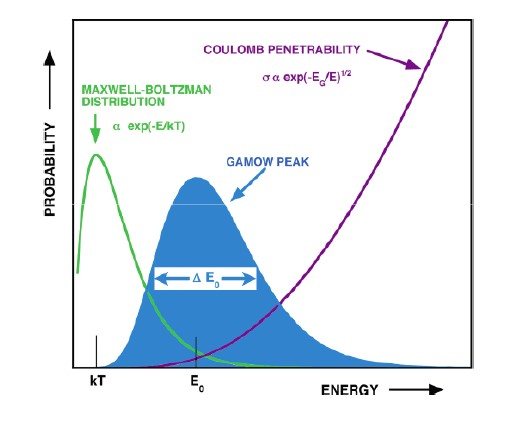
\includegraphics[scale=0.7]{Figures/gamow.jpg} 
     \caption{Κορυφή Gamow.}
     \label{fig:apx:gamow}
\end{figure}
Aν συνδυάσουμε αυτές τις δύο καμπύλες, η ενεργός διατομή γίνεται μέγιστη για τιμές ενέργειας που βρίσκονται μέσα στην μπλε περιοχή. Η καμπύλη που οριοθετεί την μπλε περιοχή ονομάζεται \textit{κορυφή Gamow} και το μέγιστο εύρος αυτής της περιοχής ονομάζεται \textit{παράθυρο ενεργειών Gamow}. Ο ρυθμός των αντιδράσεων φαίνεται, μέσα από αυτό το διάγραμμα, να είναι πιο δραστικός (effective) όταν τα σωματίδια παίρνουν τιμές ενέργειας που βρίσκονται μέσα στην μπλε περιοχή. Με αυτό τον τρόπο, μπορούμε εύκολα να διακρίνουμε ποιές τιμές ενεργειών είναι οι πιο δραστικές. Παρατηρούμε ότι τυπικά αυτές οι τιμές είναι σχετικά χαμηλές.
%------------------------------------------------------------------------------------------------------------
%------------------------------------------------------------------------------------------------------------
%------------------------------------------------------------------------------------------------------------
\section{Δίκτυο πυρηνικών αντιδράσεων}
 Ο αρχικός μας σκοπός ήταν να κατασκευάσουμε μια διαφορική εξίσωση, η αριθμητική επίλυση της οποίας θα μας προσομοιώνει την διαδικασία της πυρηνοσύνθεσης. Έτσι το επόμενο βήμα είναι να εκφράσουμε τα παραπάνω ως μια διαφορική εξίσωση της μεταβολής των αριθμητικών πυκνοτήτων συναρτήσει της χρονικής τους μεταβολής. Η ποσότητα που θέλουμε να δούμε πως μεταβάλλεται και είναι και η πιο εύκολα μετρήσιμη παρατηρησιακά, είναι η μεταβολή της αφθονίας (abundance) ενός στοιχείου, πυρήνα, σωματίου ή ισοτόπου με το χρόνο. Για να φτάσουμε όμως σε αυτό το σημείο πρέπει να κάνουμε κάποιες παραδοχές. Εκφράζουμε λοιπόν τον αριθμό των αντιδράσεων ανά μονάδα χρόνου και όγκου μέσω μιας διαφορικής εξίσωσης και βλέπουμε το πως μεταβάλλεται με τον χρόνο η αριθμητική πυκνότητα του i-σωματίου για μια αντίδραση $i(j,o)m$, δηλαδή για μια αντίδραση των $i+j$ όπου θα μας δώσει $ o+m $ σωμάτια. Θεωρώντας ότι τα $i,j$ μεταβάλλονται με τον ίδιο ρυθμό, έχουμε:
 
\begin{equation}
\label{eq60}
r_{i,j}=\frac{1}{1+\delta_{ij}}n_{i}n_{j}\langle\sigma u \rangle \longrightarrow
\end{equation} 
\begin{align}
\label{eq61_62}
\left( \frac{\partial n_{i}}{\partial t} \right)_{\rho} &= \left( \frac{\partial n_{j}}{\partial t} \right)_{\rho}= -r_{i,j} \\ \nonumber \\
\left( \frac{\partial n_{o}}{\partial t} \right)_{\rho} &= \left( \frac{\partial n_{m}}{\partial t} \right)_{\rho}= +r_{i,j}
\end{align}
Δηλάδή για κάθε αντίδραση μεταξύ των i και j, έχουμε καταστροφή των i, j και δημιουργία των ο, m. Ο όρος $\displaystyle \frac{1}{1+\delta_{ij}}$ είναι απαραίτητος στην περίπτωση που μελετάμε αντιδράσεις μεταξύ δύο ίδιων σωματιδίων και μας βοηθά να μην μετρήσουμε αυτή την αντίδραση δύο φορές. Η ποσότητα $\delta_{ij}$ δεν είναι άλλη από το δέλτα του Κronecker. Ένας πολύ σημαντικός παράγοντας όμως σε αυτόν τον συλλογισμό που πρέπει να ληφθεί σοβαρά υπόψιν είναι ότι η αριθμητική πυκνότητα ενός σωματίου εξαρτάται άμεσα από την πυκνότητα της ύλης. Έτσι, η πλήρης έκφραση της αριθμητικής πυκνότητας μιας ποσότητας είναι αυτή που δίνεται από την σχέση
\begin{equation}
\label{eq63}
\dot{n_{i}}= \left( \frac{\partial n_{i}}{\partial t} \right)_{\rho} + n_{i}\frac{\dot{\rho}}{\rho}
\end{equation}

Βλέπουμε ότι η $\dot{n_{i}}$ εκφράζεται από δύο όρους. Έναν όρο στον οποίο η παράμετρος της πυκνότητας ύλης είναι σταθερή και έναν στον οποίο εκφράζεται η μεταβολή της. Στη μελέτη μας όμως των διαδικασιών της πυρηνοσύνθεσης, η μεταβολή της αριθμητικής πυκνότητας ως προς την πυκνότητα ύλης δεν έχει μεγάλη συμβολή. Η μεταβολή που επηρρεάζει σημαντικά τη μελέτη μας είναι εκείνη η οποία μας δίνει την αλλαγής της αριθμητικής πυκνότητας, του αριθμού δηλαδή των σωματιδίων i, j κατά τη διάρκεια των αντιδράσεων. Συνεπώς, προς το παρόν θα αγνοήσουμε την ποσότητα $n_{i}\frac{\dot{\rho}}{\rho}$ και να επικεντρώσουμε την μελέτη μας στην μεταβολή των αντιδράσεων, δηλαδή του όρου $\left( \frac{\partial n_{i}}{\partial t} \right)_{\rho} $.
Για τον λόγο αυτό χρησιμοποιούμε την ποσότητα της αφθονίας ($Y=n/\rho N_{A}$) ή του λόγου μάζας ($X_{i}=A_{i}Y_{i}$). Σχετικά με τον λόγο μάζας, γνωρίζουμε ότι το άθροισμα όλων των μαζών κανονικοποιείται στην μονάδα. Έτσι, ελέγχοντας τον λόγο μάζας κατά τη διάρκεια προσομοίωσης των αντιδράσεων, βλέπουμε τις μεταβολές που έχουμε στην μάζα. Έτσι λοιπόν, όταν το άθροισμα  αυτό γίνεται μικρότερο από μονάδα ξέρουμε ότι έχουμε απώλεια μάζας και μετατροπή της κατά πάσα πιθανότητα σε ενέργεια.
Τώρα πλέον, μπορούμε να συμπεριλάβουμε στους υπολογισμούς μας και την μικρή συνεισφορά που προέρχεται από την μεταβολή της αφθονίας του σωματίου που μας ενδιαφέρει συναρτήσει της πυκνότητας ύλης. Χρησιμοποιώντας τον ορισμό της αφθονίας έχουμε
\begin{equation}
\label{eq64}
\dfrac{{dY}_{i}}{dt}=\frac{d }{dt} \frac{n_{i}}{\rho N_{A}}\Rightarrow \dot{Y}_{i}= \frac{\dot{n_{i}}}{\rho N_{A}}-\frac{n_{i}}{\rho N_{A}} \frac{\dot{\rho}}{\rho}
\end{equation}

Μπορούμε τώρα να αντικαταστήσουμε το $\dot{n_{i}}$ από το πρώτο μέλος της σχέσης \eqref{eq63} και αν θέλουμε να το εκφράσουμε με όρους σχετικούς με την θερμοπυρηνική ενεργό διατομή, θα αντικαταστήσουμε τις αριθμητικές πυκνότητες των i, j με τις αφθονίες τους. Έτσι, σε συνδυασμό με τη σχέση \eqref{eq61_62} προκύπτει ότι
\begin{equation}
\label{eq65}
\dot{Y}_{i}= \frac{1}{\rho N_{A}} \left( \frac{\partial n_{i}}{\partial t} \right)_{\rho} = - \frac{r_{i,j}}{\rho N_{A}}=-\frac{1}{1+ \delta_{ij}}\rho N_{A} \langle\sigma u \rangle _{i,j} Y_{i}Y_{j}
\end{equation}

Μέχρι τώρα στη μελέτη μας θεωρήσαμε αντιδράσεις που γίνονται μεταξύ νουκλεονίων. Στη Φύση όμως, έχουμε και αντιδράσεις που γίνονται από αλληλεπίδρασεις νουκλεονίων ή πυρήνων με φωτόνια, λεπτόνια ή νετρίνα. Επιπλέον, μέχρι τώρα δεν λάβαμε υπόψιν μας τις διασπάσεις των πυρήνων. Για να λάβουμε και αυτές τις αλληλεπιδράσεις και διεργασίες υπόψιν, ορίζουμε μια ειδική παράμετρο, την παράμετρο λ. Η παράμετρος αυτή θα πάρει τη θέση του όρου $r_{i,j}$ και η χρονική παράγωγος της αφθονίας θα έχει τη μορφή
\begin{equation}
\label{eq66}
\dot{Y_{i}}=-\lambda _{i} Y_{i}
\end{equation}
Έτσι λοιπόν, μέσω αυτής της παραμέτρου μπορούμε να εκφράσουμε τον ρυθμό των διασπάσεων (decay rates) ή αν έχουμε αντιδράσεις με λεπτόνια, φωτόνια ή νετρίνα με μια αντίστοιχη παράμετρο λ. Για παράδειγμα, αν έχουμε μια φωτοδιάσπαση ατόμων οξυγόνου $^{16}$O από φωτόνια, ο ρυθμός με τον οποίο θα γίνονται αυτές οι διασπάσεις θα εκφραστούν μέσω της λ. Αξίζει να αναφέρουμε ότι υπολογιστικά, για έναν κώδικα οι αντιδράσεις που γίνονται από την αλληλεπίδραση νουκλεονίων με φωτόνια, λεπτόνια ή νετρίνα αντιμετωπίζονται με τον ίδιο τρόπο και επηρρεάζουν την αφθονία όπως φαίνεται στη σχέση \eqref{eq66}. Σύμφωνα με τα παραπάνω, γίνεται σαφές ότι οι αλληλεπιδράσεις που μπορούν να λάβουν χώρα χωρίζονται σε  δύο κατηγορίες

\begin{itemize}
\item Mεταξύ δύο πυρήνων ή νουκλεονίων.
\item Μεταξύ πυρήνων/νουκλεονίων και φωτονίων, λεπτονίων, νετρίνων - διασπάσεων.
\end{itemize}

Φτάνοντας πλέον πολύ κοντά στην τελική γραφή της ζητούμενης διαφορικής εξίσωσης που θέλουμε να λύσουμε έχουμε να κάνουμε λίγες σκέψεις ακόμα.
%------------------------------------------------------------------------------------------------------------
%------------------------------------------------------------------------------------------------------------
%------------------------------------------------------------------------------------------------------------
\section{Αντίστροφες Αντιδράσεις}
Αντίστροφες (inverse) είναι οι χημικές αντιδράσεις κατά τις οποίες τα αντιδρώντα μετασχηματίζονται  σε προϊόντα σε έναν χρόνο t αλλά αν αντιστρέψουμε αυτόν το χρόνο και πάμε να δούμε τι αντίδραση γίνεται σε -t, η αλληλεπίδραση των προϊόντων θα μας δώσει σαν αποτέλεσμα τα αρχικώς αντιδρώντα. Για παράδειγμα, αν μέσα στον αστέρα αντιδράσει ένας  $^{12}$C με ένα σωμάτιο α ($^{4}$He) θα δώσει ένα οξυγόνο ($^{16}$O) και ένα φωτόνιο-γ αλλά και το αντίστροφο. Για να μελετήσουμε αυτές τις αντιδράσεις, θα πρέπει να ξαναγράψουμε την ενεργό διατομή για μια αντίστροφη αντίδραση η οποία θα έχει τη μορφή:

\begin{equation}
\label{eq67}
\langle \sigma u \rangle _{i,j,o} = \frac{1+\delta_{ij}}{1+\delta_{om}} \frac{G_{m}g_{o}}{G_{i}g_{j}} \left(  \frac{\mu_{om}}{\mu_{ij}} \right) ^{3/2} \exp \left( -Q_{o,j}/kT \right) \langle \sigma u \rangle_{m,o,j}
\end{equation}

Στην τελευταία σχέση βλέπουμε τον τύπο της θερμοπυρηνικής ενεργού διατομής για την κατεύθυνση $\langle \sigma u \rangle _{i,j,o}$ και στο τέλος, την θερμοπυρηνική ενεργό διατομή για την αντίστροφη κατευθυνση $\sigma u \rangle_{m,o,j}$. Όπως παρατηρούμε, αυτές οι δύο διατομές σχετίζονται. Ο εκθετικός όρος $Q$ εκφράζει την ενεργειακή διαφορά μεταξύ αντιδρώντων και προϊόντων (άρα και το είδος της αντίδρασης, αν είναι δηλαδή ενδόθερμη ή εξώθερμη) και ο πρώτος όρος εκφράζει την πυκνότητα καταστάσεων και τη συνάρτηση επιμερισμού του συστήματος που μελετάμε. Αυτό σημαίνει για τους υπολογισμούς μας ότι αν μετρήσουμε την ενεργό διατομή για μια κατεύθυνση --πειραματικά ή και θεωρητικά μέσω κάποιου μοντέλου-- και αν γνωρίζουμε επίσης την συνάρτηση επιμερισμού του συστήματος και την τιμή της $Q$, μπορούμε εύκολα να υπολογίσουμε την ενεργό διατομή της αντίστροφης κατεύθυνσης μέσω της τελευταίας σχέσης.

\section{Θεμελιώδης Διαφορική Εξίσωση}
Συνδυάζοντας όλα τα παραπάνω, είμαστε πλέον σε θέση να γράψουμε με σαφήνεια και λαμβάνοντας υπόψιν όλες τις σημαντικές παραμέτρους, την θεμελιώδη διαφορική εξίσωση που μπορεί στη συνέχεια να μας βοηθήσει να προσομοιώσουμε τις διαδικασίες της πυρηνοσύνθεσης, η μορφή της οποίας είναι

\begin{align}
\label{eq68}
\nonumber \dot{Y} &= \sum_{j} N^{i}_{j} \lambda_{j} Y_{j}+ \sum_{j,k} N^{i}_{jk}\rho N_{A} \langle\sigma u \rangle _{jk}Y_{j}Y_{k} + \\ \nonumber \\
&+ \sum_{j,k,l} N^{i}_{jkl}\rho ^{2} N_{A} ^{2} \langle\sigma u \rangle _{jkl}Y_{j}Y_{k}Y_{l}
\end{align}
Έτσι, για κάθε πυρηνικό είδος που θέλουμε να μελετήσουμε, έχουμε μια διαφορική εξίσωση που μπορεί να μας βοηθήσει η οποία μοιάζει με την σχέση \eqref{eq68}. Καθώς λοπόν μεταβάλλεται με το χρόνο η αφθονία ενός είδους, βλέπουμε ότι αυτή η μεταβολή εξαρτάται απ' όλες τις αλληλεπιδράσεις που εμπλέκονται και συμβάλλουν στην δημιουργία ή την καταστροφή του i-στοιχείου. Συνήθως, ομαδοποιούμε τους όρους ανά είδος αντιδράσεων. Έτσι, στην εξίσωση \eqref{eq68} ο πρώτος όρος εκφράζει τις αλληλεπιδράσεις του i-στοιχείου με φωτόνια, λεπτόνια, νετρίνα ή πιθανές διασπάσεις, ο δεύτερος εκφράζει τις αντιδράσεις μεταξύ των i-στοιχείων. Οι όροι $N$, είναι ουσιαστικά μετρητές σωματιδίων και μας πληροφορούν για το πόσα σωματίδια δημιουργούνται ή καταστρέφονται από την κάθε αλληλεπίδραση. Ο τρίτος όρος τώρα, εκφράζει την περίπτωση εκείνη όπου στην αντίδραση συμμετέχουν περισσότερα από δύο σωμάτια, όπως είναι η περίπτωση της αντίδρασης τρία-α. Σε μια τέτοια αντίδραση πρέπει να μετρήσουμε την θερμοπυρηνική ενεργό διατομή και του τρίτου σωματίου καθώς και την αφθονία του. Εξαιτίας τώρα των 3 αφθονιών έχουμε τους όρους της πυκνότητας και του αριθμού Avogadro υψωμένους στο τετράγωνο. 
Απ' αυτό το σημείο και μετά, είμαστε σε θέση, λαμβάνοντας υπόψιν μερικές παραμέτρους ακόμα σχετικά με τα αστροφυσικά φαινόμενα στα οποία έχουμε πυρηνοσύνθεση καθώς και τα επιμέρους χαρακτηριστικά της κάθε διαδικασίας, να μελετήσουμε υπολογιστικά την πιθανή εξέλιξη και προέλευση των διαφόρων βαρέων --και όχι μόνο-- χημικών στοιχείων.

